\section{Exo-parasite}

\begin{rpg-commentbox}{Exo-parasite}
    The parasite is a scorpion like creature with four strong legs a tail ending on a powerful sting and a huge maw under its bely. The maw and stings on the creature's legs have powerful neurotoxin able to jeopardize a host's motor abilities. The host is lethargic, yet still alive and in the moments it is not under the effects of the toxin, it can feel the creature tentacles moving though your organs and slowly feeding from your corpse. 
\end{rpg-commentbox}    


\begin{rpg-commentbox}{}

    \centering{\textbf{Stats}}

    \par\noindent\rule{\textwidth}{0.4pt}

    \textbf{SPEED} 2

    \textbf{HEALTH}: 2

    \textbf{SKILLS}: Mobility 8, Observation 8
    
    \textbf{ARMOR}: 2 (0 vs fire)
    
    \textbf{ACID SPLASH}: 4

    \par\noindent\rule{\textwidth}{0.4pt}

    \begin{small}
    \begin{enumerate}
        \item SKITTERING MENACE The parasite has chosen its host and they know it is coming for
        them! It skitters forward, single-minded and horrifyingly spider-like. The victim suffers +1
        STRESS LEVEL and must make an immediate Panic Roll.
        \item same as above
        
        \par\noindent\rule{.9\textwidth}{0.4pt}

        \item TAIL LASH The little monster comes for its target, lashing out with its wicked tail. It attacks
        with five Base Dice, Damage 1.

        \par\noindent\rule{.9\textwidth}{0.4pt}

        \item TAIL GRAPPLE: The parasite leaps and catches its victim from behind, its tail whipping
        violently. Roll a D6:
            1–2: The target’s legs are caught and they fall prone — make a Panic Roll.
            
            3–4: The victim’s arms get hopelessly tangled in the beast’s tail — they cannot use any held items and must make a Panic Roll.
            
            5–6: The parasite wraps its tail around the target’s neck, choking them — they suffer the effects of DROWNING and must make a Panic Roll. 

        \par\noindent\rule{.9\textwidth}{0.4pt}

        \item SPINE GRAPPLE The parasite leaps at its victim. Make an opposed roll with six Base Dice
        against the target’s CLOSE COMBAT skill (not counting as an action for the victim):
            If the parasite wins, the target will suffer THE FINAL EMBRACE (below) on the parasite's next initiative.

            If the victim wins they throw the beast to the floor, but it’s not finished with them
        yet and attacks the same target again on its next initiative. 

        \par\noindent\rule{.9\textwidth}{0.4pt}

        \item THE FINAL EMBRACE The parasite gets to its victim, its acid making short work of any armor or respirator in the way. Roll for the attack with six Base Dice. If it gets one or more, the poor victim is hugged and immediately Broken.
    \end{enumerate}
    \end{small}

\end{rpg-commentbox}

\begin{rpg-commentbox}{Host}
    While attached to a host, the creature seeks a quiet place where it can fully merge its DNA with the host, dropping the empty shell and taking full control of the host. If attacked, first deduce any damage from the host. If the host dies, the creature detaches and it will try to escape or attach itself to a new host.
    While attached, substitute 5s and 6s with:

    \par\noindent\rule{.9\textwidth}{0.4pt}

    ALL-OUT ATTACK: The exo-parasite launches into a wild attack, throwing every one of its sting legs at its victim. It attacks with eight Base Dice, Damage 1.

\end{rpg-commentbox} 


\begin{figure}
    \centering
    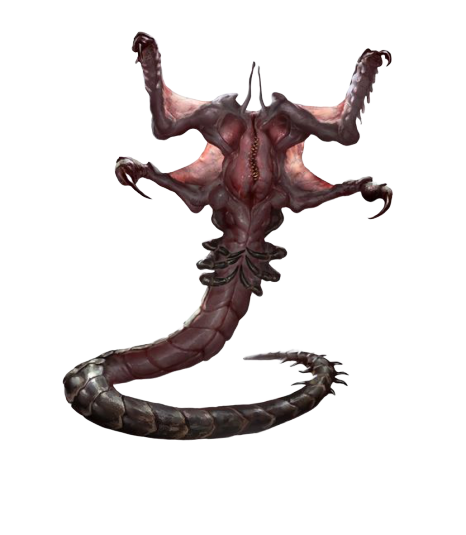
\includegraphics[width=.45\textwidth]{img/stage-I-bg.png}
    \label{fig:stage-1}
    \caption*{Stage I - Exo-parasite}
\end{figure}
